
\subsection{Research Field Classification}
\label{section:field_classification}
\subsubsection{Task Description}
The goal of this task is to identify the research fields covered in social science publications.
In general, two approaches could be applied to this task. One is the extraction of relevant terms of the publications. It means that this task could be seen as a keyword extraction task and the detected terms considered as descriptive terms regarding the research field. The second approach is to learn to classify publications research fields with the use of annotated data. The advantage of the second approach is the usage of classes of topics which could be generated by experts of domains. Therefore, we would have well-defined categories.

Since we didn't recieve any gold standard ---annotated training data--- for this task, we decided to train a classifier using annotated data from SSOAR.
In this way, our interpretation of the task is to select one or more labels from a given set of labels for each publication. This approach is known as a mulit-label classification. In our case, a label represents a research field.

\subsubsection{Our approach - Overview }
The annotated data of SSOAR contains four different annotation schemes for research field related information. By reviewing these schemes, We decided to use the Classification Social Science (classoz)annotation scheme. The number of classes in each schema, coverage of each classification, and the distribution of data in each schema affected our decision. 
Because SSOAR is a multilingual repository and the publications given by the RCC are mainly English, we need to select English training data.
In a first step we selected all metadata records which include an English abstract and a classoz annotation.
After this filtering 22,453 records are left over.

Due to the unequal distribution of labels in the dataset, we need to guaranty enough training data for each label.
We selected only labels with frequency over 300 for training the model which results in a total of 44 out of 154 classification labels representing research fields.
We decided to train a classification model based on the fasttext framework~\cite{joulin2017bag}. To train our model we resort to the abstracts of the publication, as this approach worked better than using the full-texts.

\subsubsection{Evaluation}

For creating train and test set, 22,453 SSOAR publications with their assigned labels were split randomly. 10\% of data formed test set and rest of data went to train set. As it is mentioned a fasttext model trained with learning rate 1.0, epoch 150. Also, negative sampling parameter is set to 25.  In this experiment, only the top 3 labels with the highest probabilities were considered for the evaluations.

Figure~\ref{fig:results_fasttext} shows the performance of the model regarding various evaluation metrics for different thresholds. A label is assigned to a publication if the model outputs a probability for the label above the defined threshold. In multi-label classification, this allows us to evaluate our model from different perspectives. As it is illustrated in figure~\ref{fig:results_fasttext}, the point that the micro precision curve and micro recall meet is at threshold of 0.1. We can see the point as the highest point of micro f1-measure. By increasing the threshold from this point, micro precision score is increasing but micro recall is falling. By Decreasing threshold, these trends are opposite.  Also, the default threshold doesn't look promising. In spite of micro precision about 0.7, we have a problem with the very high number of items without any prediction. 


%The x-a  the change of  metrics over different probability thresholds for generating the result.
\begin{comment}

This graph shows the change of different evaluation metrics over different probability thresholds for generating the result. 
The threshold defines the minimum probability of a label which is leading to an assignment.

Orderly, micro precision and micro recall values are 0.5 for threshold 0.1
For this threshold, the model generates a prediction for all items and about half of the items have at least one correct prediction. 
All these metrics remain the same till threshold 0.2. Till threshold 0.6, we can see a dramatic increase in the micro precision and the number of items without any correct prediction. Both of these metrics pass 0.8. On the other hand, micro recall falls to the below of 0.2. In this case, selecting threshold seems hard task, since the conflict point of precision and recall is a threshold about 0.25 but both of these metrics at the point are not more than 0.3 and also we have more than 0.4 items with completely wrong predictions. Also, the default threshold doesn't look promising. In spite of micro precision about 0.7, we have a problem with the very high number of items without any prediction.
\end{comment}

\begin{figure}[t]
\centering
%\subfloat[Random Forest Evaluation]{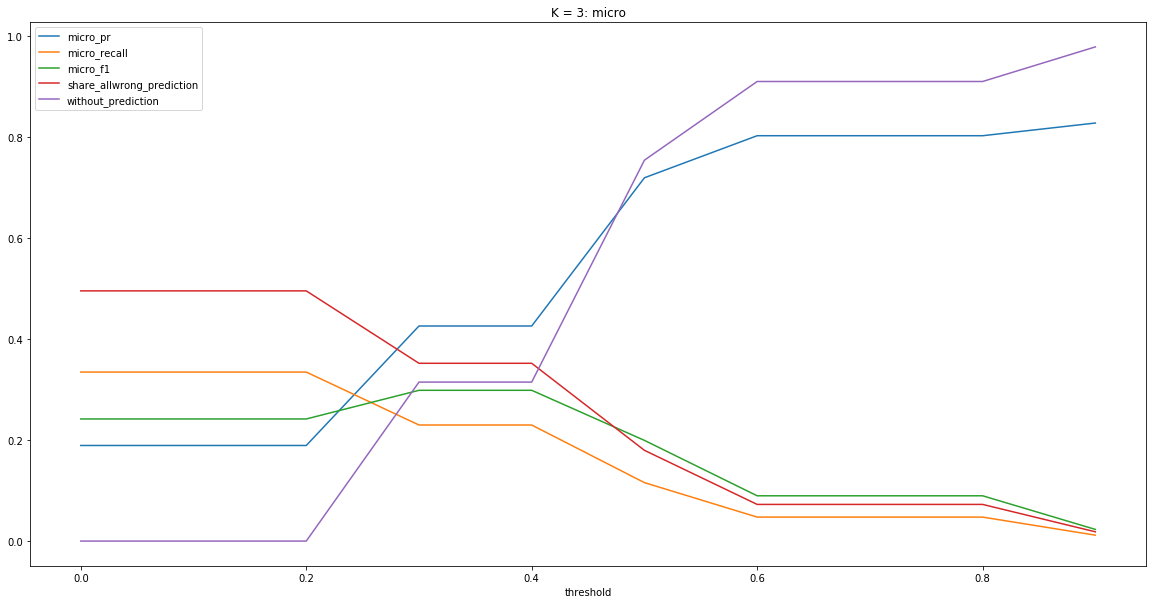
\includegraphics[width=0.49\textwidth]{figures/research-fields/random-forest-evaluation.png}\label{fig:rf}}
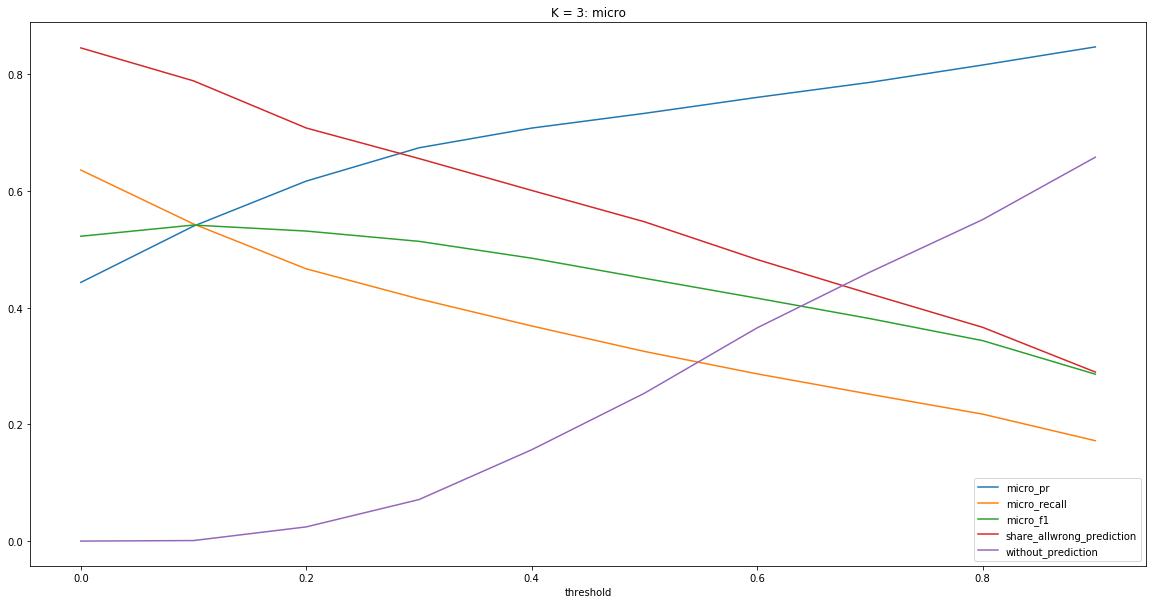
\includegraphics[width=0.49\textwidth]{figures/research-fields/fast-text-evaluation.png}
%\vspace{-1em}
\caption{Precision-Recall vs. Threshold}
\label{fig:results_fasttext}
\end{figure}



%The trends of micro f1, micro recall, and publications with just wrong predictions are falling smoothly, but the trend of micro precision and number of publications without any prediction are rising gradually. 
%The Micro precision still is higher than 0.7 for threshold 0.4. Also, the number of items without prediction is lower in threshold 0.4 than threshold 0.5 (the difference is about 0.1).

% We also experiment with random forest 



%purple curve (without_prediciton) 
%The measure without_prediction describes the share of publications without any prediction at all.
%E.g. if we only accept predicted labels with a model certainty of 60\%, 40\% of the publication have no predictions. 

%red curve (share_allwrong_prediction)
%The red curve describes the share of documents in the test set, which contain only wrong predictions for each threshold.
%This means when a threshold of 20\% certainty is selected 70\% of the publications have only wrong predictions. But if a threshold of 80\% certainty is selected only 40\% of the publications have only wrong predictions. 
